\begin{block}{Historic Cold Snaps}
    Visualizing temperature anomalies facilitates identification of large-scale weather patterns superimposed on long-term climatological averages.
    We compare the February 2021 cold snap (bottom row) to four historic cold snaps.
    \begin{framed}
        \begin{figure}
            \centering
            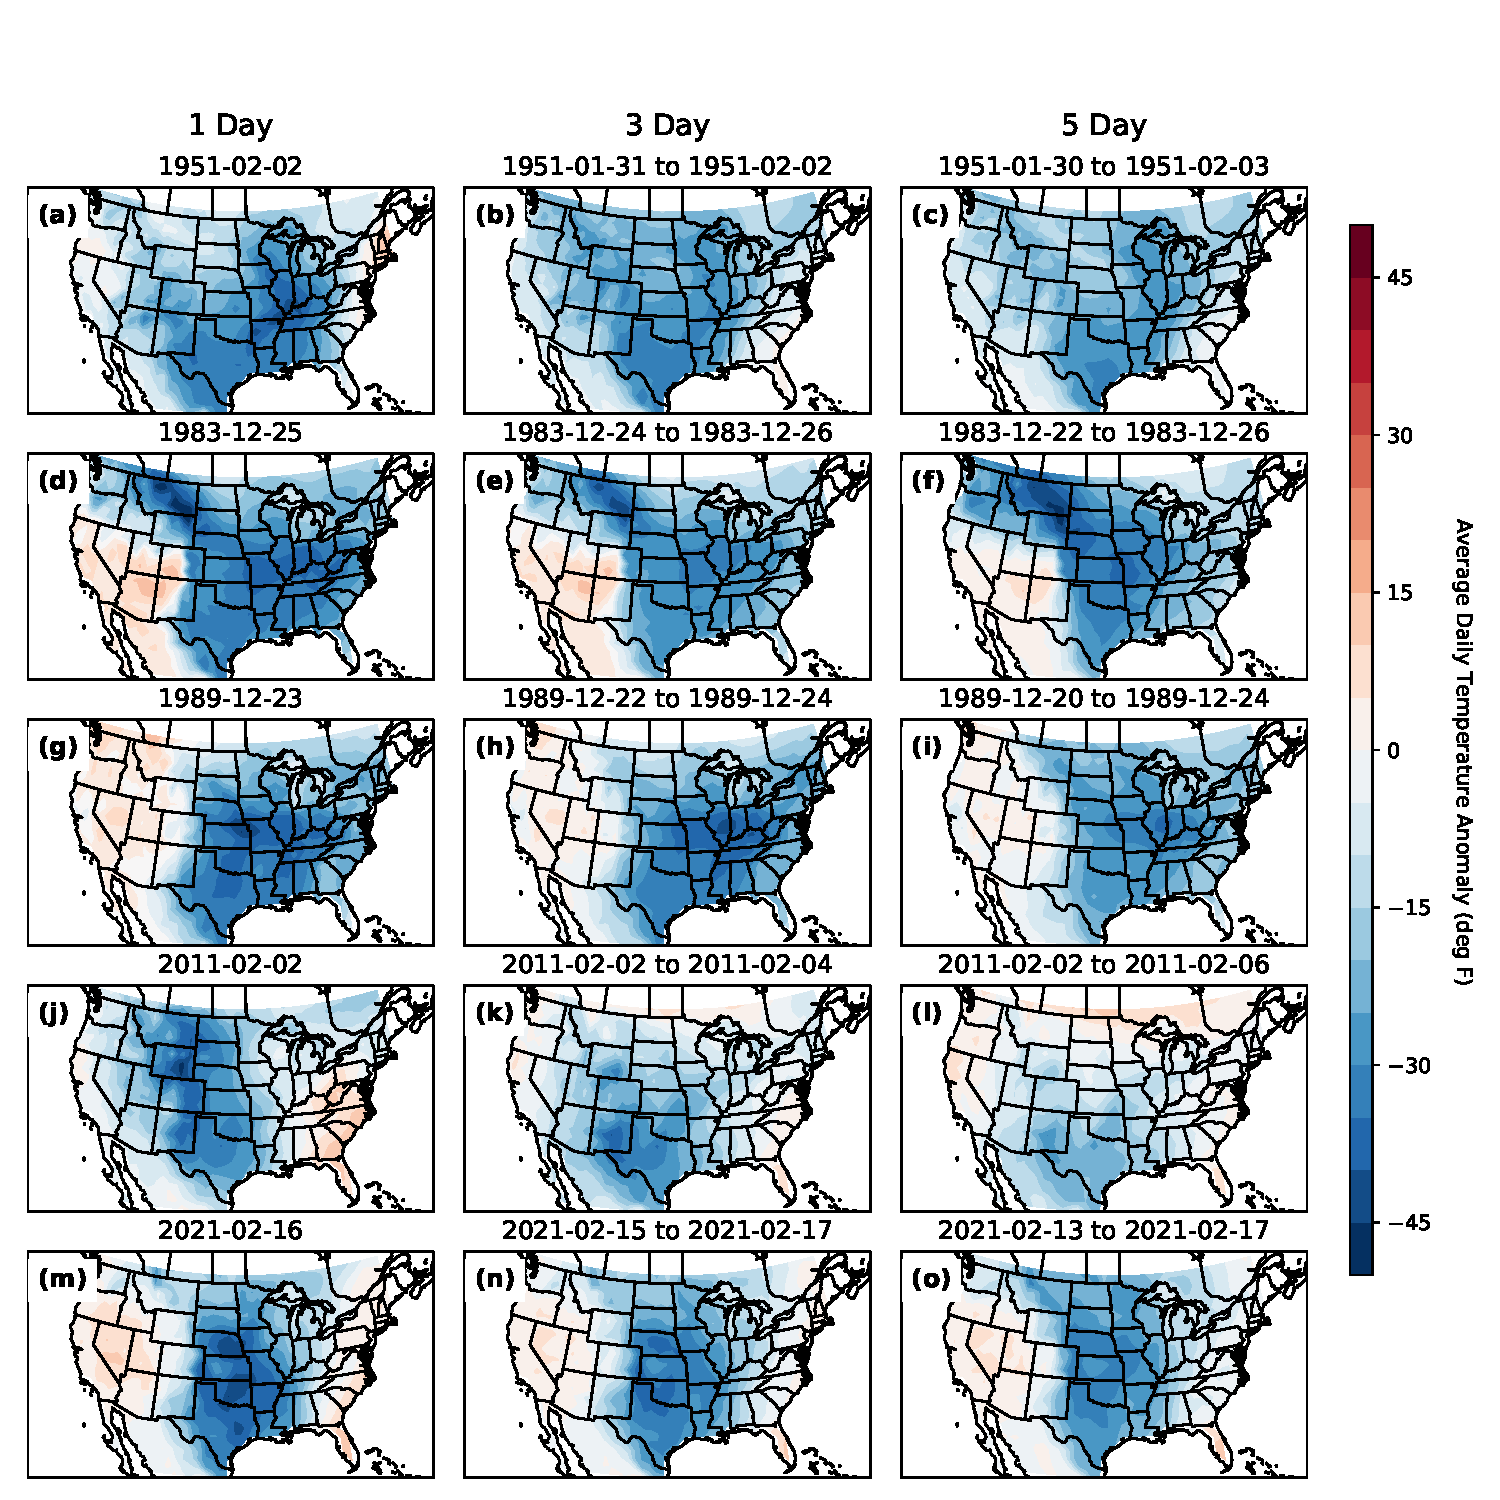
\includegraphics[width=\textwidth]{historic_events_era5.pdf}
            \caption{
                Anomalies of daily mean temperatures from the ERA-5 reanalysis \cite{hersbach_era5:2020} during previous cold snaps demonstrate a qualitative precedent for severe cold.
            }\label{fig:historic_era5}
        \end{figure}
    \end{framed}
\end{block}